\chapter{The LHC complex and the CMS experiment}
\label{chapter:cms}

In this Chapter a brief description of the Large Hadron Collider and of the CMS detector are
presented in order to contextualize the physics analyses that are described in the following chapters.
In particular, the CMS subdectors are described, since they are fundamental for the reconstruction of particles,
such as photons and products of partons hadronization.

\section{The Large Hadron Collider}

The Large Hadron Collider (LHC) is the largest and most energetic machine ever build to study
matter at the subatomic scale. It is operated by CERN and is located at the boarder between France and
Switzerland close to Geneve. It collides protons up to a center of mass energy of 13 TeV.

The LHC is located underground ($\sim 100$ m below the surface) and has a total lenght of about 27 km.
The tunnel that houses the LHC was previously occupied by the Large proton electron collider (LEP) that
played a crucial role in investigating the properties of the Z and W bosons.

The primary goal of LHC has been to study the electroweak simmetry breaking through first discovery of the Higgs boson and later
precision measurements of the its properties.
The energies explored by the collisions at LHC allow to probe the standard model up to scales of few TeV where
interactions not described by the SM could be observed in various production and decay processes.

The same machine is also used to accelarate and collide proton with ions or ions with ions.

The design of the LHC aims to reach a center of mass energy of 14 TeV and an istantaneous luminosity ($\mathcal{L}$)
of $10^{34}cm^{-2}s^{-1}$ for $p-p$ collisions. The scientific program span several decades, in the current phase it will
deliver to the experiments about $300 \fbinv$ of integrated luminosity, while it will reach $3000 \fbinv$ during the dacade
starting in 2025 (Figure~\ref{fig:lhc_plan}). 

\begin{figure}[!h]
  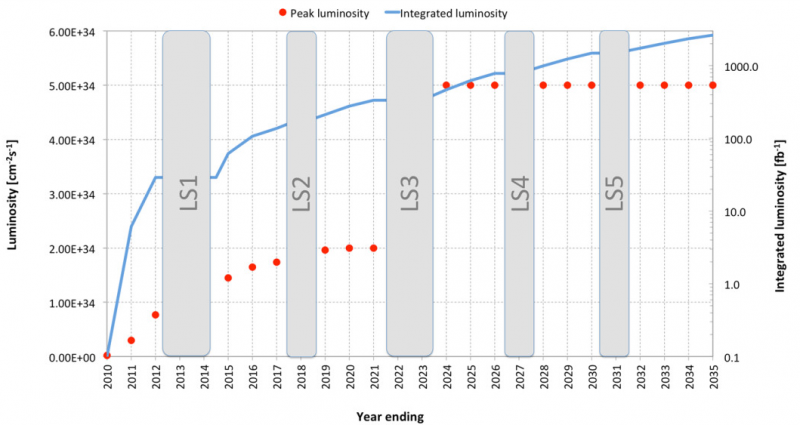
\includegraphics[width = 1.\textwidth]{figures/cms/Projected_LHC_Performance.png}
  \caption{Illustration of the foreseen LHC schedule, the current phase ends with long shutdown 3 (LS3). The high
    luminosity phase (HL-LHC) starts after LS3 and will last for a decade. LHC standard operation includes running
    periods during spring, summer and fall and a technical stop for small upgrades and mantainance during winter.
    Larger upgrades are carried out during long shutdowns (LS), a major one will be the upgrade of the LHC and of
  the experiments during LS3.}
  \label{fig:lhc_plan}  
\end{figure}

\section{LHC properties}
The high beam intensities necessary for reaching the design luminosity make the
use of two separate proton beams necessary. The collision of two beams of equally charged par-
ticles requires opposite magnet dipole fields in both beams. The LHC is therefore designed as a
proton-proton collider with separate magnet fields and vacuum chambers in the main arcs, with 
common sections only at the insertion regions where the experiments are located.
The choice to reach at regime centre of mass energies of 14 TeV has forced to have a mag-
netic field of $\sim 8.3$ T, requiring 9300 liquid Helium cooled superconducting magnets made of a
Niobium-Titanium compound at a temperature of 1.9 K, by means of super-fluid Helium. Figure \ref{fig:lhc_chain}
shows all the acceleration steps the particles have to perform in order to reach 14 TeV
energies. 

\begin{figure}[!h]
  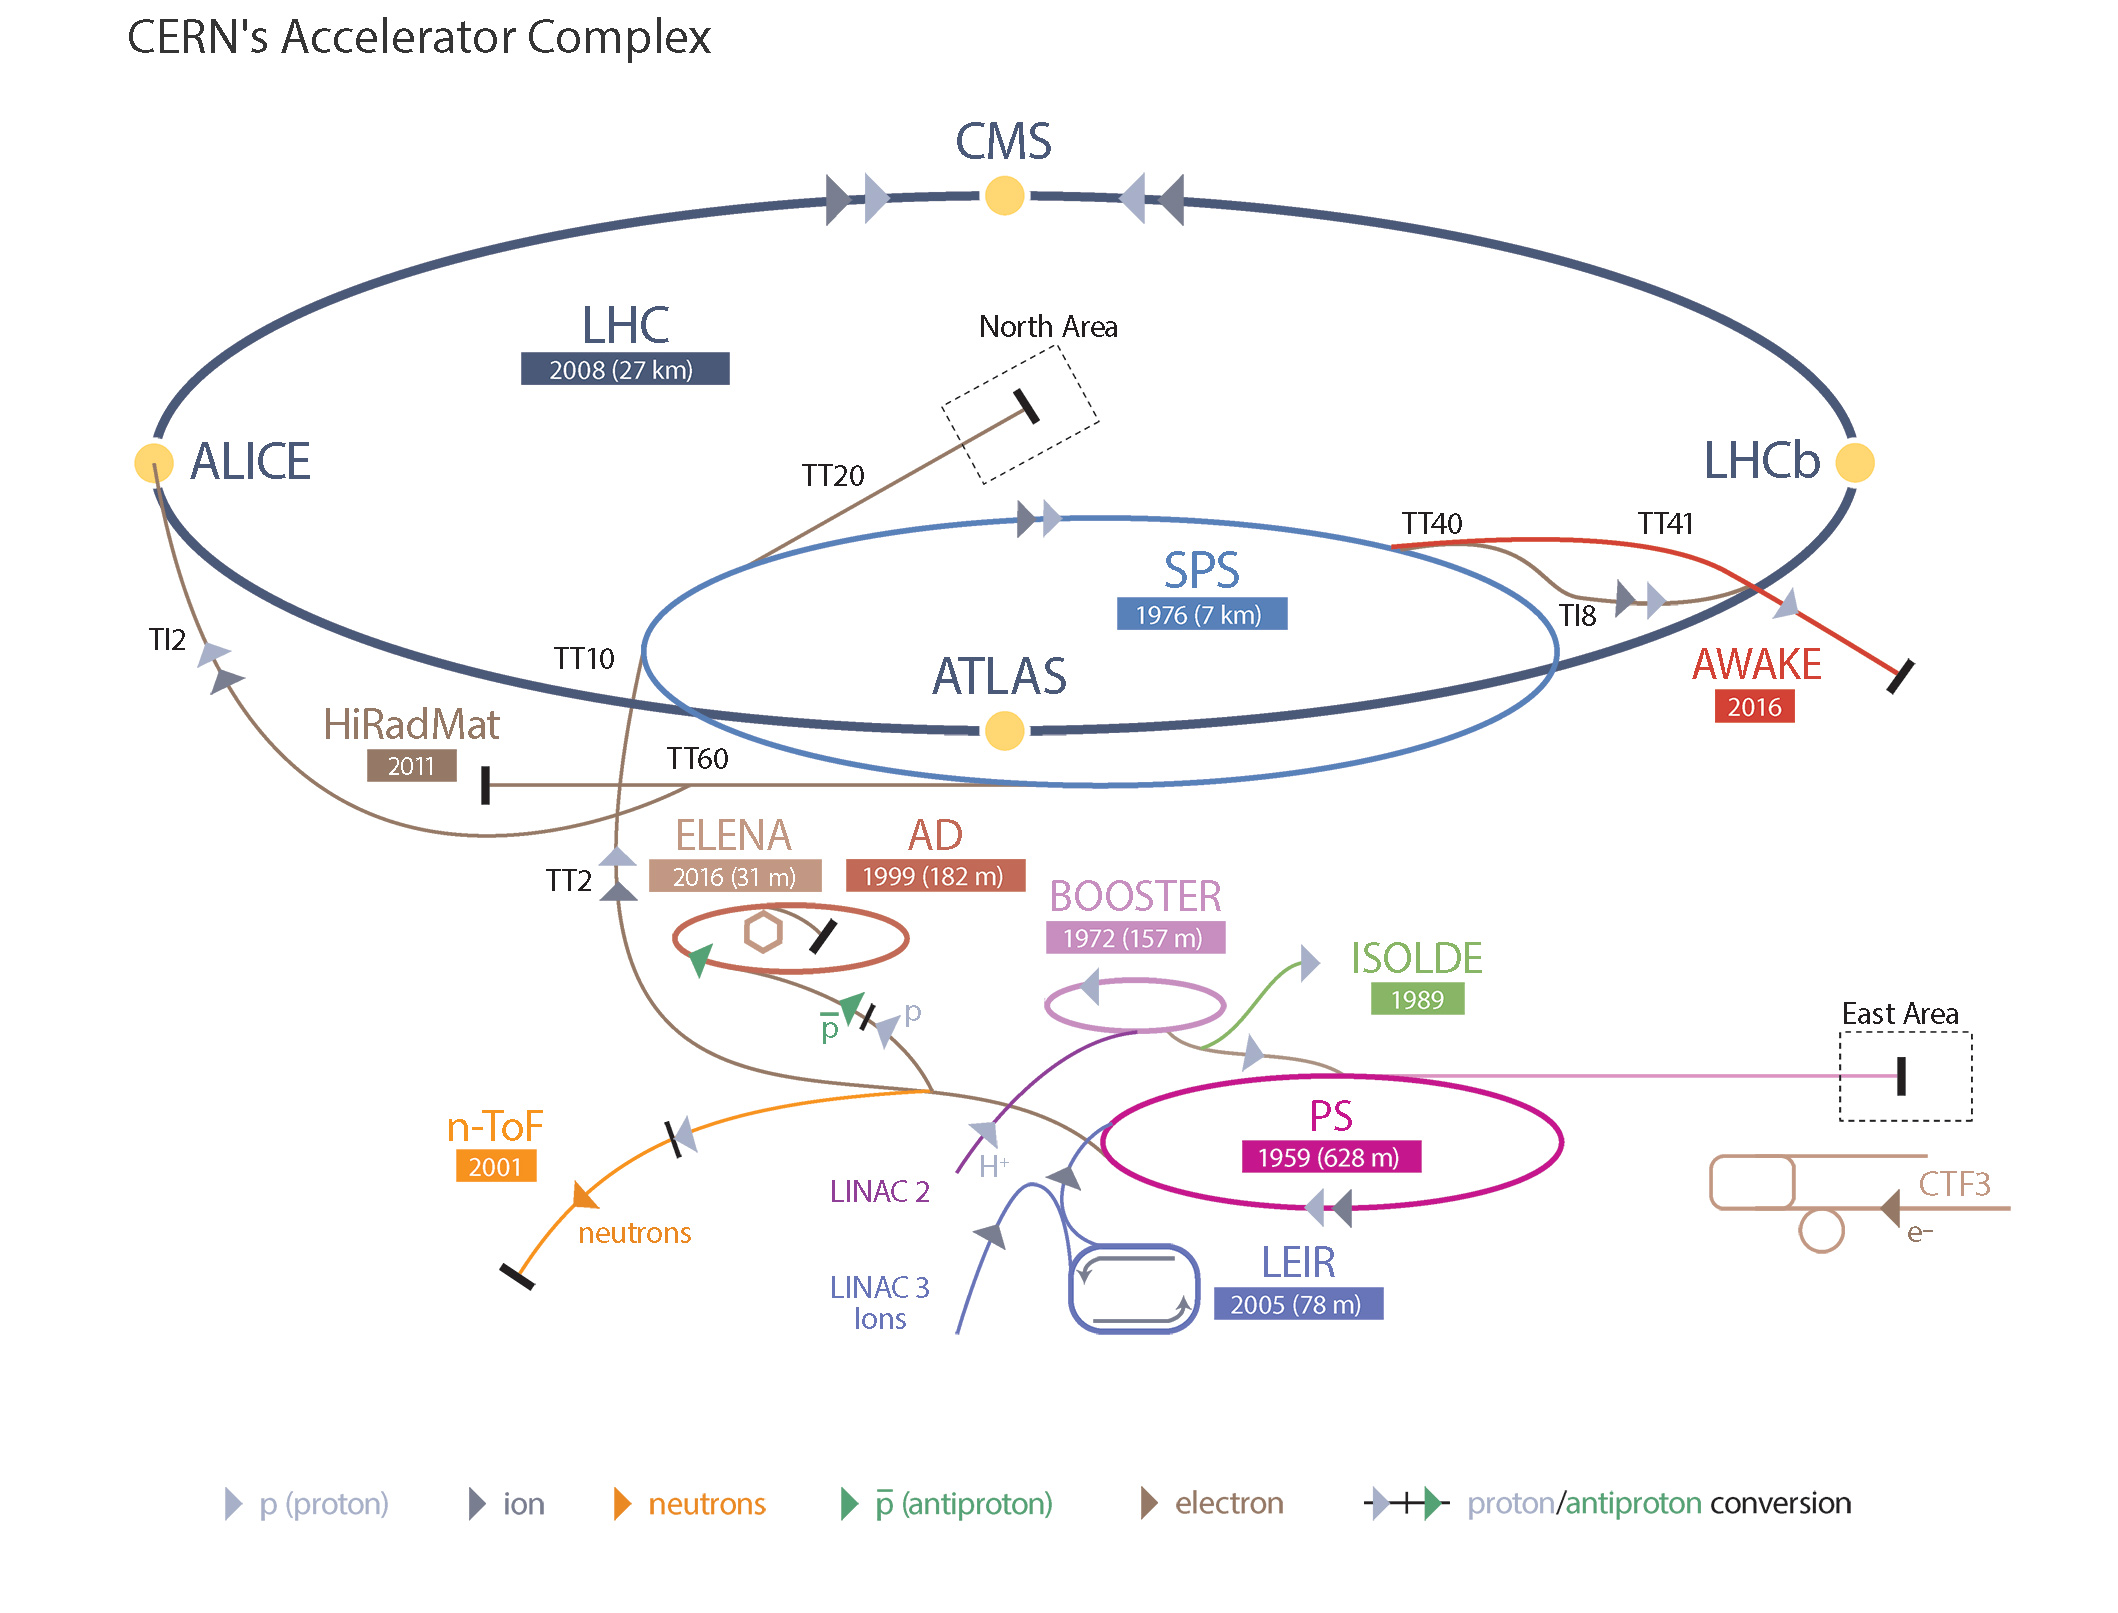
\includegraphics[width = 1.\textwidth]{figures/cms/LHC_accelarator_complex.jpg}
  \caption{The CERN accelerators complex. Protons are first extracted from a hydrogen tank and and accellarated up to 50 MeV by
    a linear accelarator (Linac 2), the Proton syncroton booser (BOOSTER) and Proton syncroton (PS) push the energy up to
    1.4 GeV and 25 GeV respectively. Protons are then transfered to the Super proton syncroton (SPS) where they are accelerated to
    450 GeV and injected into the LHC. Others machines are present at CERN complex to provide dedicated beams to various experiments.
    Furthermore both from the PS and the SPS the proton or ion beam is sent to a fixed target to provide secondary beams of pions, muons and electrons to several areas dedicated to fixed target experiments or R\&D projects. 
  }
  \label{fig:lhc_chain}  
\end{figure}

To reach the nominal luminosity, up to 2808 bunches per beam, with about $1.1\times 10^{10}$
protons each, are collided every 25 ns.
On the LHC ring four main experiments are located: ATLAS~\cite{atlas}, CMS~\cite{cms}, LHCb~\cite{lhcb} and
ALICE~\cite{alice}. CMS and ATLAS are general purpose experiments, with complementary features
and detector choices. CMS is described in detail in the next sections. The LHCb collaboration
aim to perform precision measurements on CP violation and rare decays, in order to reveal
possible indications for new physics phenomena. ALICE is dedicated to heavy ions physics and the
goal of the experiment is the investigation of the behaviour of the strongly interacting hadronic
matter resulting from high energy lead nuclei collisions. In those extreme energy densities the
formation of a new phase of matter, the quark-gluon plasma, is expected.

The LHC cycle consists of several phases: the machine is filled with protons while the energy is kept at
450 GeV, once the machine is full the beams are accelerated, squeezed and set on colliding orbits.
The instantaneous luminosity is maximized in ATLAS and CMS while in ALICE and LHCb it is kept
at lower values. Each cycle is called a ``fill''.

\section{The CMS experiment}

The CMS experiment is a general purpose detector for particle physics. The detector
includes several subsystems symmetrically centered around
the fifth interaction point of LHC. The detector is 22 m long and 15 m wide and is depicted in Figure~\ref{fig:CMS}.
It consists of a central, ``barrel'', part and two forward regions, the ``endcaps'', which
detect particles at small deflection angles.
The main detector component is the is the
superconducting solenoid that generate a magnetic field of 3.8 T. The tracking and calorimeter
systems are contained within the solenoid. This design benefits
the particle reconstruction as it minimizes the probability for a charged particle to
generate a shower before reaching the calorimeters while traversing the dense material of
the solenoid. Most of the detector is supported by
a steel skeleton which serves also as the return yoke for the magnetic field of 1.8 T
present outside the solenoid volume.
The muon detection system is placed outide the solenoid and inside the return yoke. The CMS detector has a weight
of about 12500 tonnes, mainly due to the steel skeleton and the solenoid.

\begin{figure}[!h]
  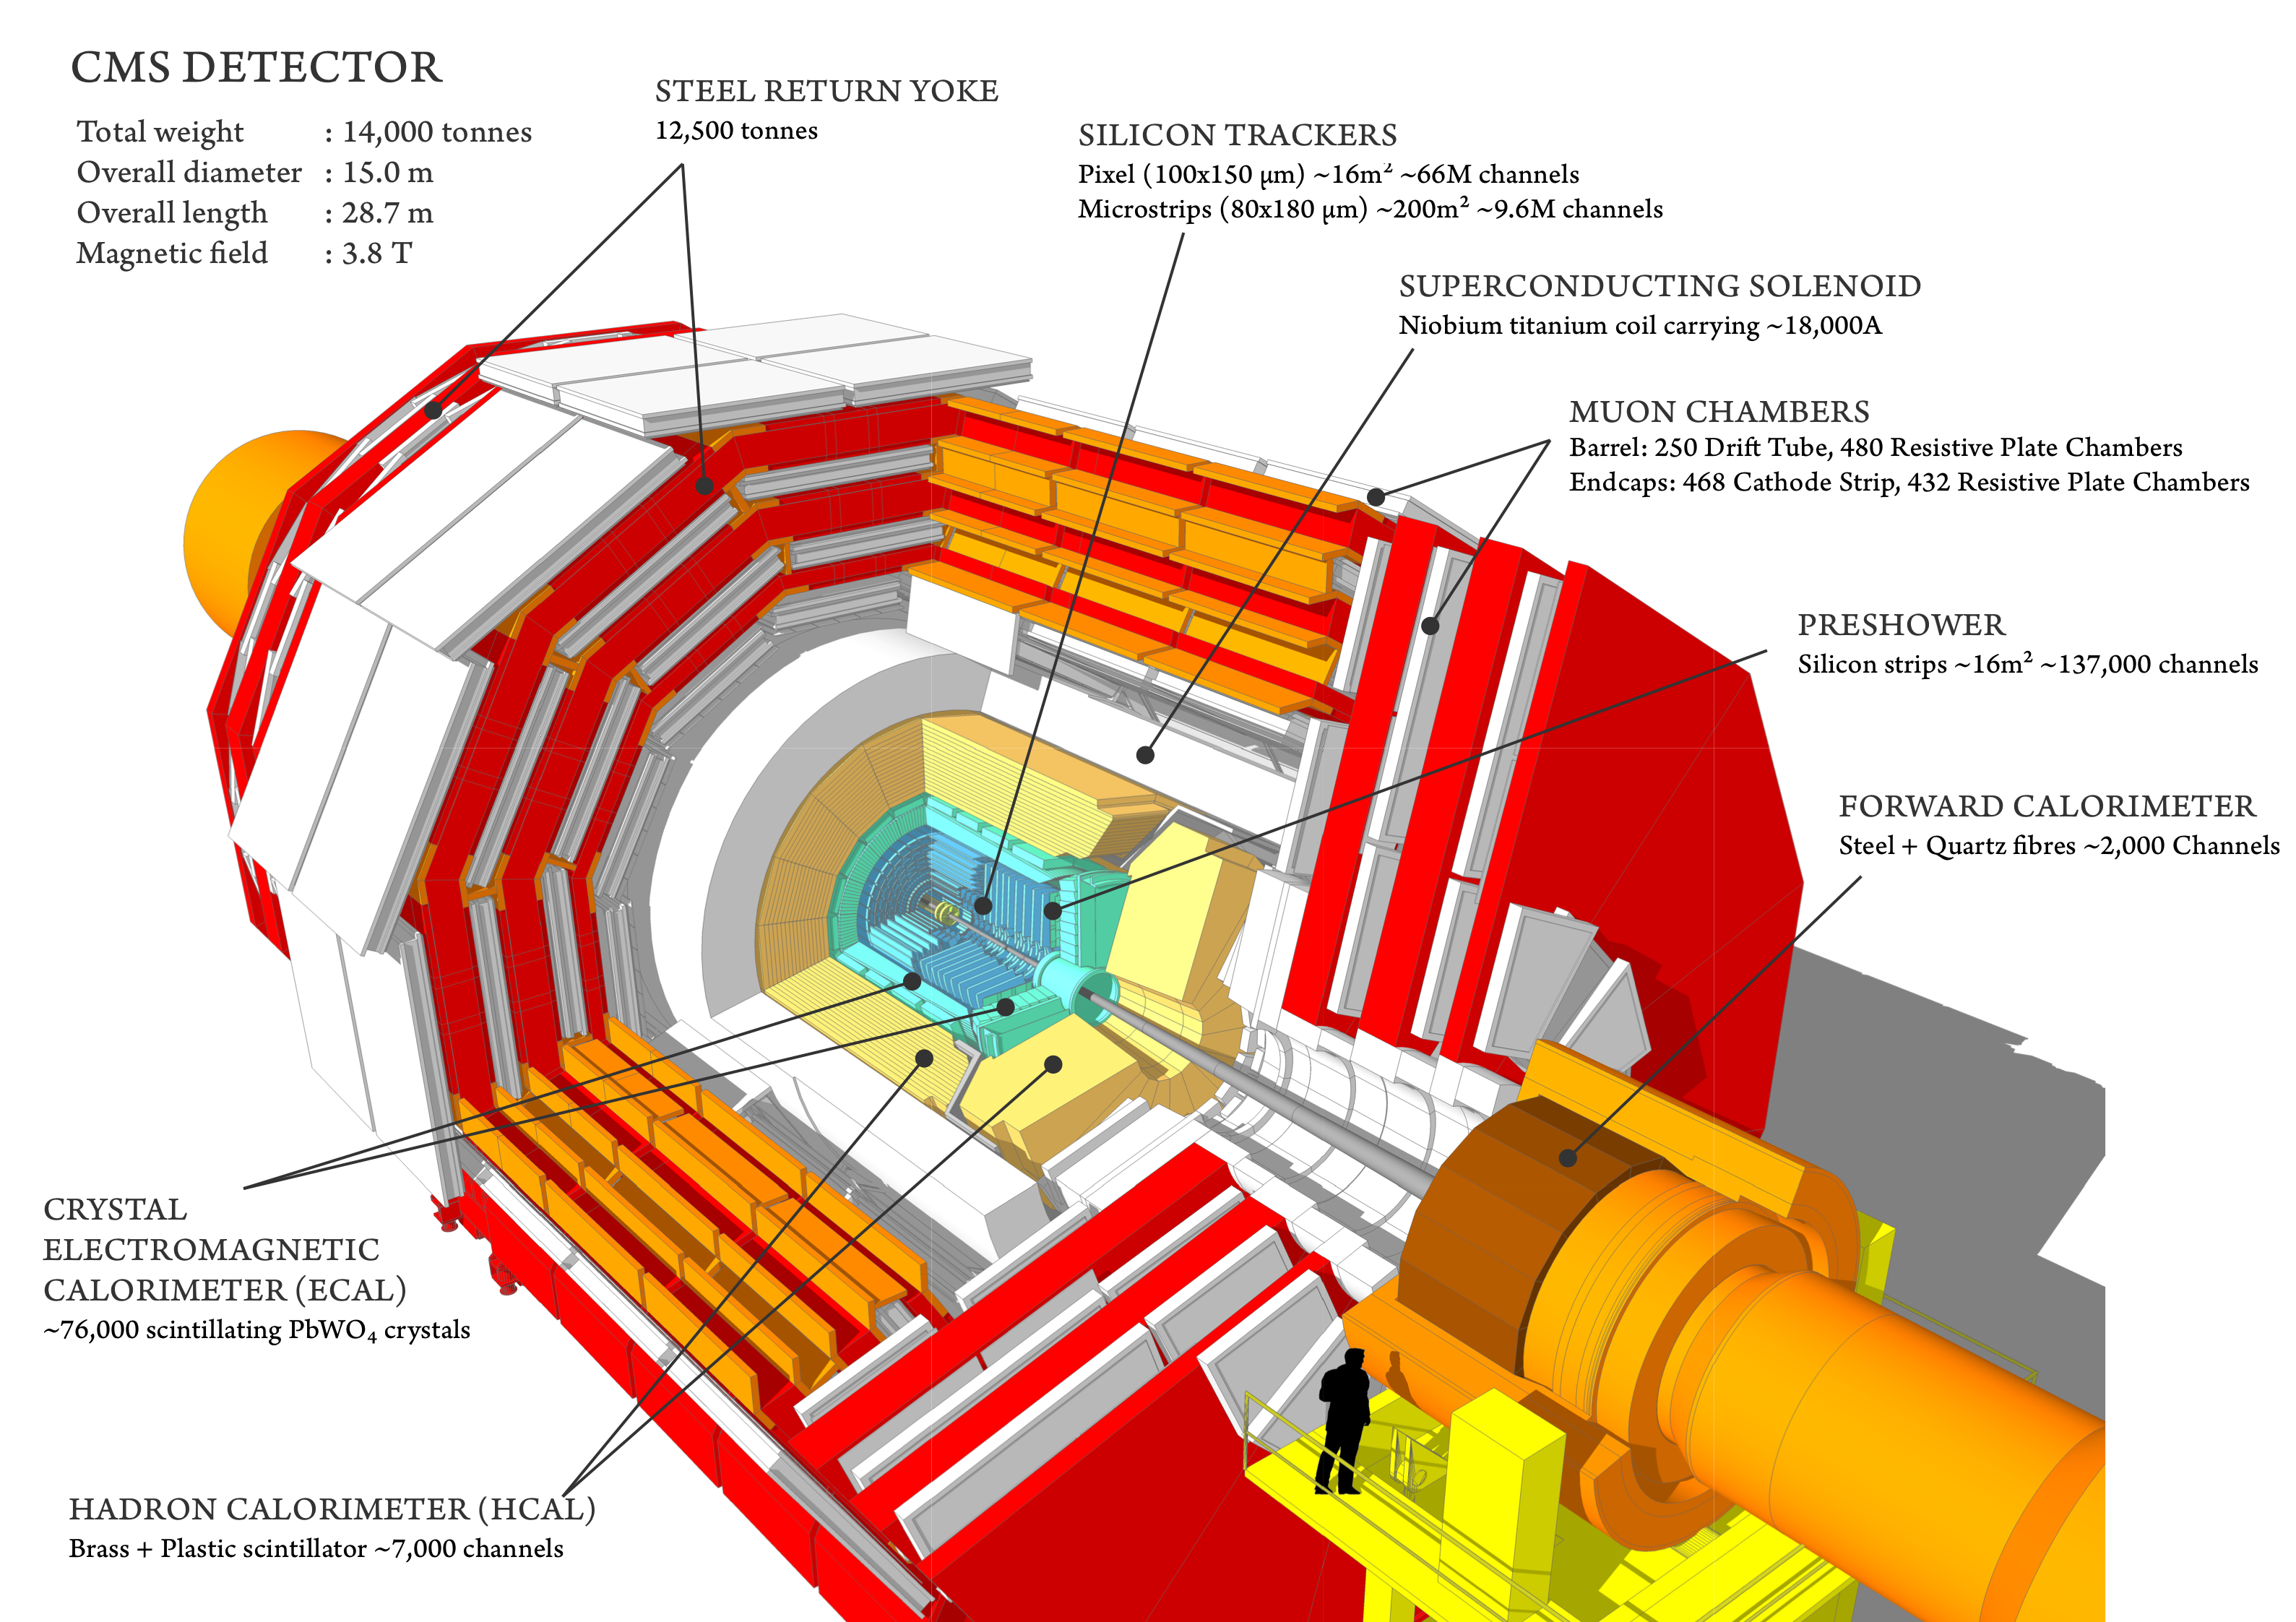
\includegraphics[width = 1.\textwidth]{figures/cms/cms_layout.png}
  \caption{Sketch of the Compact Muon Solenoid experiment \cite{cms_sketch}.}
  \label{fig:CMS}  
\end{figure}


The origin of the right-handed coordinate system of CMS is the central collision point,
with the z-axis oriented in the anticlockwise-beam direction. The x-axis is oriented
towards the center of the LHC accelerator ring, the y-axis points upwards.

The azimuthal angle ($\phi$) lies in the x-y plane and is measured
from the x-axis. A slice of the CMS detector in this x-y plane is shown in Figure~\ref{fig:CMS_xycut}.
The polar angle ($\theta$) is directed upwards from the z-axis. With the polar angle, the
pseudorapidity ($\eta$) can be defined:

\[
\eta = -ln( tan( \frac{\theta}{2} ) )
\]

The paricle mass $m$, momentum in the transverse plane $p_T$ and its $\eta$ and $\phi$ rappresent a convinient set of
variables to describe the particles produced in hadronic $p-p$ collisions where the fraction
of momentum carried by each of the colliding parton is in principle unknown.

\begin{figure}[!h]
  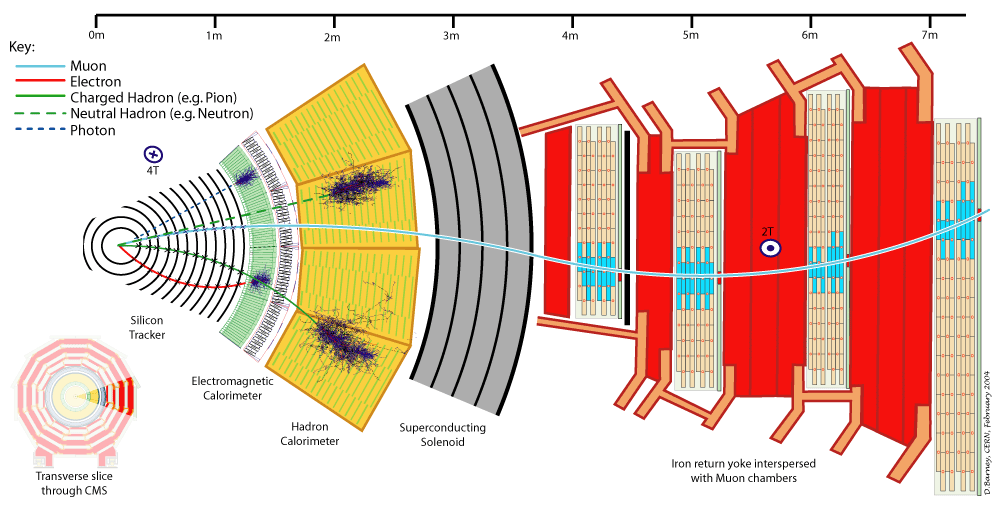
\includegraphics[width = 1.\textwidth]{figures/cms/CMS_Slice.png}
  \caption{A slice of the CMS detector in the x-y plane. Various particle type detection are depicted, the
    details of each system are given in the text.}
  \label{fig:CMS_xycut}  
\end{figure}

\subsection{The tracking system}
The tracking detector surrounds the beampipe, the innermost layer is installed
about 4 cm from the interaction point (IP). It has a length of 5.8 m, a diameter of 2.6 m,
and covers a range of $|\eta| < 2.5$ with an area of over $200~\mathrm{m}^{2}$ active silicon sensors, its
layout is shown in Figure~\ref{fig:cms_tracker_layout}. It is
designed to measure the trajectories of particles as highlighted in Figure~\ref{fig:CMS_xycut}. As such,
it has to provide a high spatial resolution and a fast signal readout while withstanding a fluence
of about $10^6$ particles/( cm$^2$ s) (at a distance of 8 cm from
the IP).
The core of the tracking system, the silicon pixel detector, is made of 66 million pixels
with a size of $100 \times 150 \mu$m$^2$ , enabling the reconstruction of primary and secondary
vertices with a precision that ranges between 100 $\mu$m to 1 mm in the z direction and of few tens of $\mu$m
in the x and y directions. The silicon pixel detector is followed by a silicon strip detector with coarser
granularity. The track recognition is performed by about 15200 highly sensitive
modules containing 10 million detector strips. The tracking detector has a radiation length ($X_0$) of 0.4 at $\eta = 0$,
which increases at larger $\eta$ to approximately 1.8 $X_0$ at $|\eta|$ = 1.4 as visible from Figure~\ref{fig:cms_tracker_material}.

\begin{figure}[h]
  \centering
  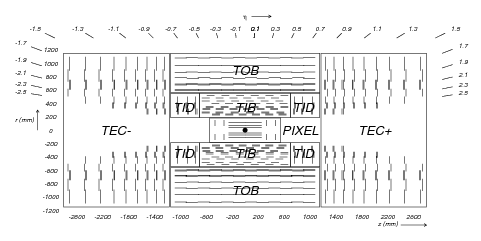
\includegraphics[width = 1.\textwidth]{figures/cms/trackerLayout.png}
  \caption{Schematic cross section through the CMS tracker in the r-z plane. Each line-element represents a detector module.
    Closely spaced double line-elements indicate back-to-back silicon strip modules,
    in which one module is rotated through a ``stereo'' angle, so as to permit reconstruction of the hit positions in
    three dimensions. Within a given layer, each module is shifted slightly in r or z with respect to its neighbouring modules,
    which allows them to overlap, thereby avoiding gaps in the acceptance \cite{cms_trk}.}
  \label{fig:cms_tracker_layout}
\end{figure}

\begin{figure}[h!]
  \centering
  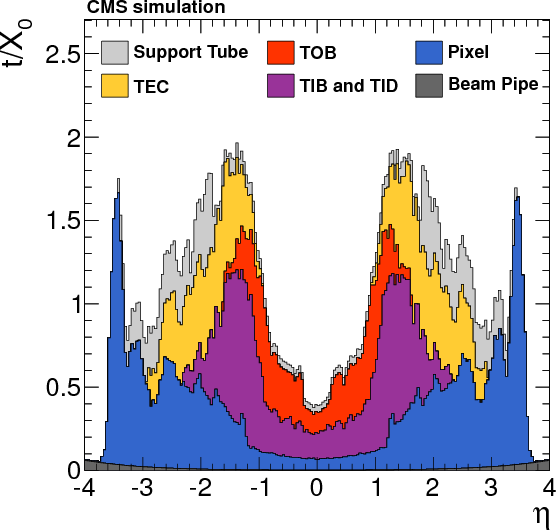
\includegraphics[width = .7\textwidth]{figures/cms/MaterialBudget.png}
  \caption{Total thickness $t$ of the tracker material traversed by a particle produced at the nominal interaction point,
    as a function of pseudorapidity $\eta$, expressed in units of radiation length $X_0$.
    The contribution to the total material budget of each of the subsystems that comprise the CMS tracker is shown,
    together with contributions from the beam pipe and from the support tube that surrounds the tracker~\cite{cms_trk}.
    The configuration shown in the picture reflects that of the CMS tracker prior the upgrade of the
    pixel detector in 2017, that significantly reduces the material budget in forward region.}
  \label{fig:cms_tracker_material}
\end{figure}

\subsection{The calorimeter system}
\label{sec:cms_calo}
The calorimeter system is devided in two section: the electromagnetic part ECAL which measures the energy
of electrons and photons and the hadronic part dedicated to the measurment of the energy of charged and
neutral hadrons. The two detectors differ both in porpouse and technology.

The ECAL is an homogeneous and hermetic calorimeter, made of scintillating lead tungstate
crystals. The chosen crystal is suitable for operation at LHC due to its fast emission
(80\% of the scintillation light is emitted within 25 ns) and its resilience to irradiation. Moreover,
thanks to crystal short radiation length ($X_0 = 0.89$ cm) and small Molière radius ($r_M = 21.9$
mm), most of an electron or photon energy can be collected within a small matrix of crystals.

As the other CMS sub-detectors the ECAL is devided in two main section:
\begin{itemize}%[label=\color{black}\textbullet]\itemsep5pt
\item Barrel (EB): it covers the region $|\eta| < 1.4442$ with 61200 crystals arrenged in 170 rings of 360 crystals each.
\item Endcap (EE): it covers the region $1.556 < |\eta| < 3.0$ with 14648 crystals arrenged in 4 Dees of 3662 crystals each.
\end{itemize}

All the crystals are mounted with a tilt of $3^{\circ}$, both $\eta$ and $\phi$ projections, in
a quasi-projective geometry to avoid gaps aligned with the particles trajectories. The EB
is located at $R = 1.3$ m from the IP while the endcaps are installed at $z = \pm 3.10$ m Figure~\ref{fig:cms_ecal_layout}.

\begin{figure}
  \centering
  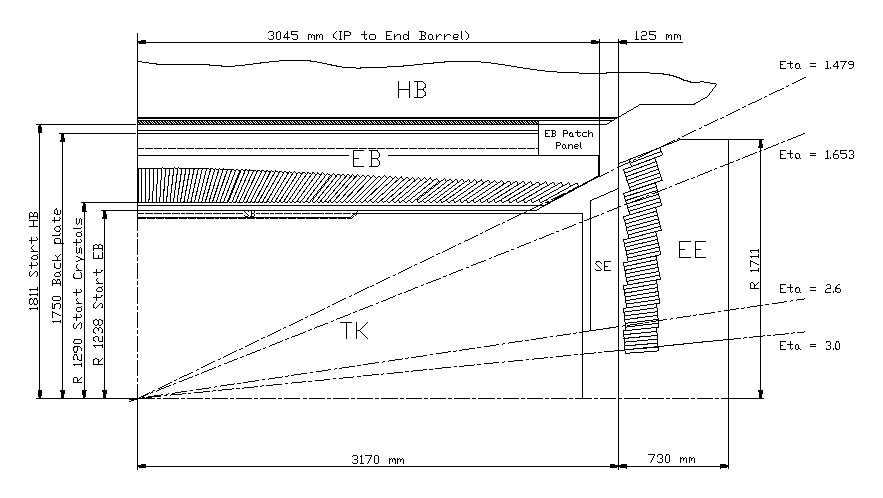
\includegraphics[width = 1.\textwidth]{figures/cms/ecal_layout.eps}
  \caption{Schematic view in the r-z plane of the CMS electromagnetic calorimeter and pre-shower. Only one fourth of the
    entire system is shown. Only the \PbWO crystals are drawn, without the supporting frame, cooling and readout
    electronic boards \cite{cms_ecal}.}
  \label{fig:cms_ecal_layout}
\end{figure}    

The relatively low light yield of $\sim 30 \gamma/$MeV makes the use of intrinsic high-gain
photodetector necessary, capable of operating in an high magnetic field. Avalanche PhotoDiodes (APDs) are
used to collect light in barrel crystals while Vacuum PhotoTriodes (VPTs) are used in the endcaps.
Two APDs are glued on the crystals rear face and their signals are summed before reaching the front-end electronics.
In the endcaps only one VPT is used for each crystal.

APDs have a gain of 50 at nominal operation bias voltage, while the relative gain variation due to changes in the bias voltage
is of $\Delta G/\Delta V = 3.1\% /V$. The APDs gain also depends on temperatures as
$\Delta G/\Delta T = -2.4\% /C^{\circ}$. 

VPTs are more radiation resilient and thus were chosen as photodector in the endcap regions
but have a gain variation of about $25\%$ across the endcaps.

ECAL operates with a temperature of $18 C^{\circ}$ which is maintained by a dedicated cooling system.
The temperature dependence of the crystal light yield ($−2\% C^{\circ}$) and of the APD gain
demand a precise temperature stabilization to the level of $0.05 C^{\circ}$ in the EB. In the
endcaps, the dependence of the VPT response on the temperature is negligible,
so a stabilization at the level of $0.1 C^{\circ}$ is sufficient. These specifications limit the contribution
of temperature variation to the constant term of the energy resolution to be less than 0.2$\%$.

The ECAL system is complemented by a pre-shower (ES) placed in front of each of the ECAL endcaps.
The ES is made two layers of silicon strips alternated with passive layers of lead radiators ($2 X_0$ and $1 X_0$)
that extend from $\eta$ 1.6 to 2.8.
The ES is used to discriminate between collimated photons caming from decays of neutral hadrons and
real photons.


The HCAL measures the energy of hadrons by stopping them within its
hermetic volume and reading out the deposited energy. Its dimensions (Figure~\ref{fig:cms_hcal_layout})
are constrained by the ECAL ($R = 1.77$ m) and the surrounding magnet coil
($R = 2.95$ m). The chosen design is the one of a sampling calorimeter with brass absorbers
and scintillating tiles for the energy measurement. The readout is performed via
optical fibers by hybrid photodiodes.

\begin{figure}
  \centering
  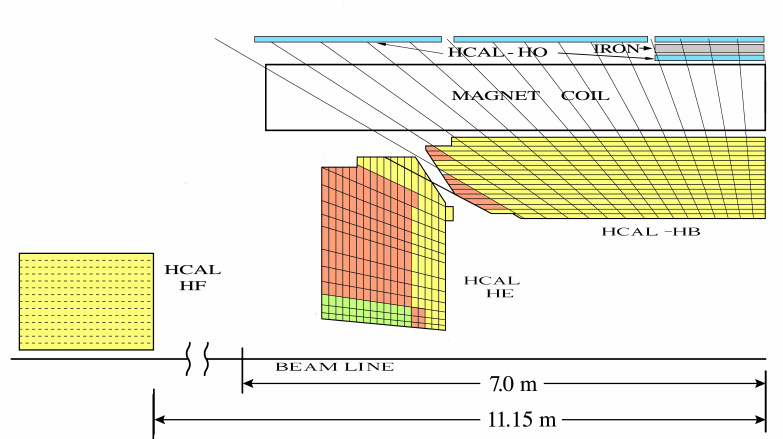
\includegraphics[width = 1.\textwidth]{figures/cms/hcal_layout.png}
  \caption{Schematic view in the r-z plane of the CMS hadronic calorimeter. Only one fourth of the
    entire system is shown. All four partitions are visible: the barrel and endcaps part (HB and HE), the
    tail catcher installed outside the CMS solenoid and the forward calorimeter.}
  \label{fig:cms_hcal_layout}
\end{figure}    

The HCAL effective thickness increases with polar angle as $1/cos\theta$ in the barrel, 
it varies from 5.82 interaction length at $\eta = 0$ to 10.6 at $\eta = 1.3$ while it is
costant at about 10 interaction length in the endcap regions.
An additional  small hadron
calorimeter is placed behind the solenoid to capture very high energetic hadrons showers not
contained with the inner calorimeters and the magnetic coil, this additional piece of the HCAL
is used to reduce the mis-identification of hadronic jets as muons. The
granularity in the barrel region ($|\eta|<1.3$) is $\Delta\eta × \Delta\phi = 0.087 \times 0.087$, while
in the endcap regions ($1.3<|\eta|<3.0$) it is
$\Delta\eta × \Delta\phi = 0.17 \times 0.17$. The forward region ($3.0 < \eta < 5.2$)
is covered by a Cherenkov-based calorimeter (HF), the absorber is made of steel while the
active medium are quartz fibers.
This forward calorimeter is placed at a distance in z of 11.2 m from the IP it has been design
to withstand 10 MGy of absorbed dose and is expected to last for ten years during the LHC operation.

\subsection{The muon system}
The CMS muon system~\cite{muon_tp} provides full geometric coverage for muon measurement up to $|\eta| = 2.4$.
The detectors are embedded in the magnet return yoke, so that muon momentum and charge
measurements can also exploit the strong magnetic return field (Figure~\ref{fig:cms_muon_layout}).
This is particularly important
for muons with transverse momentum in the $\sim 1$~TeV range, for which the complementary tracker
measurements degrade.

\begin{figure}
  \centering
  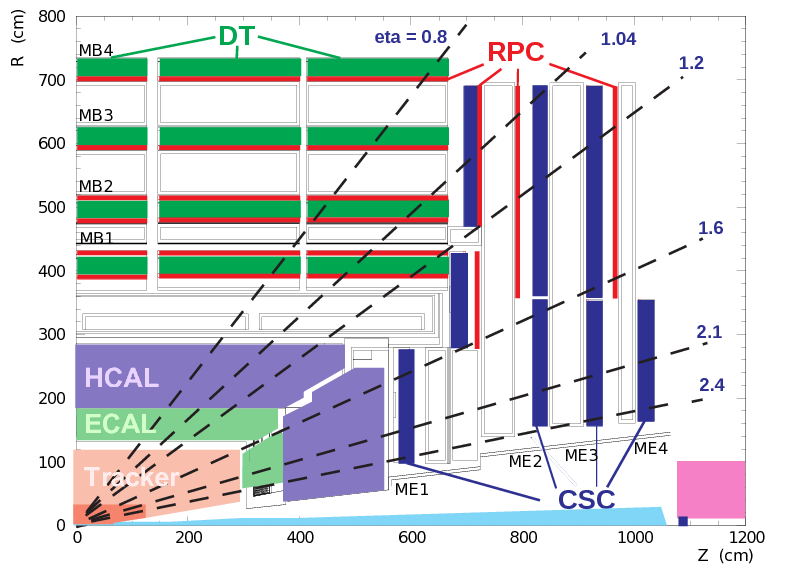
\includegraphics[width = .45\textwidth]{figures/cms/muon_layout.png}
  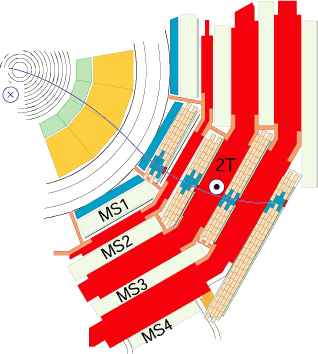
\includegraphics[width = .45\textwidth]{figures/cms/muons_xyview.png}
  \caption{Layout of one quadrant of CMS in the longitudinal (left) and transverse (right) planes.
    The four DT stations in the barrel (MB1-MB4, green),
    the four CSC stations in the endcap (ME1-ME4, blue), and the RPC stations (red) are shown.}
  \label{fig:cms_muon_layout}
\end{figure}

The CMS muon spectrometer exploit three different detector tecnologies; the need of a fast response for
generate a muon trigger and that of high spatial resolution for excellent momentum determination could not
be satisfied by a unique technology.
Both in the barrel ($|\eta| < 1.2$) and endcaps $0.9 < |\eta| < 2.4$ resistive-plate-chambers (RPC) are used
to signal the presence of high energy muons at trigger level (up to $|\eta| < 2.1$).
Drift-tube (DT) and chatode-strip-chambers (CSC) based detectors
provide the mmomentum measurement in the barrel and endcaps respectively. The angular resolution
in $\phi $ is of about 1 mrad.

The RPC and DT detectors are alternated in concentric rings at a radius between 4 and 7 m from the IP
in the barrel region. The rings are arranged in a way that avoids geometrical gaps in the $\phi $ projection, gaps
in the $\eta $ one are avoided by placing the detectors parallel to the z-axis.
In the endcaps the CSC are alternated to the RPC detectors in six consecutive disc on each side of the IP, the CSC
detectors inner region is placed at a radius of 1 m from the beamline.

\subsection{The trigger system}
The collision rate (40~MHz) is higher that the rate at which event can be recorded and stored for
offline processing (1~kHz). A two stage trigger system has been implemented to select events containing
a possible hard scattering within the tens of concurrent collisions happening at each bunch-crossing.

The first level (Level-1 trigger) is hardware  implemented in the readout electronics of each sub-system except for
the tracker. The hardware used is based custom chips programmed with a dedicated firmware.
The Level-1 triggers involve the calorimetry and muon systems, as well as some correlation
of information between these systems. The Level-1 decision is based on the presence of trigger
primitive objects such as photons, electrons, muons, and jets above adjustable transverse energy thresholds.
It also employs global sum of $E_T = \sqrt{m^2 + p_T^2}$ and $E_T^{miss}$~\cite{trigger}. Reduced-granularity and
reduced-resolution data are used to reconstruct trigger candidates.
The Level-1 trigger reduces the event rate to 100~kHz.

The second level (high level trigger or HLT) reduces the rate to the 1 kHz and performs a simplified and faster
version of the final event reconstruction. The main idea is run the event reconstruction on demand in cascade for
different types of objects such that non-interesting events can be discarded without running the whole
event reconstruction. The HLT runs on commercial CPUs, 
a set of different trigger algorithm are implemented such that the events are classified accordinlgy
to their topology (i.e. events with a muon pair, electron pair, large $E_T^{miss}$, ...).

In addition to triggers where all events that satisfies the requirements are saved (unprescaled
triggers), a set of utility triggers, whose rate would be too high due to band saturation, have
been developed, where a good event is saved only once every N times (prescaled triggers, with
a prescale parameter N). These trigger paths are used for detector studies and to study kinematical
regions of object reconstruction, such as low $p_T$ leptons.

\subsection{The event reconstruction}
\label{sec:cms_pf}
Events selected by the HLT trigger are stored and analyzed on a world-wide network of computers.
Events can be reconstructed several times if a better calibration of the detector or reconstruction algorithm is
developed. The CMS event reconstruction core is the so called particle-flow algorithm~(PF)~\cite{PF}. The PF main idea
is to combine information coming from the different systems, for instance charged hadrons are detected both
in the tracker as tracks and by the HCAL as energy deposit. Combining the momentum measurement of the tracker
with the energy measurement of the HCAL improves the overall energy resolution on hadronic jets.
Electrons and photons are primarly reconstructed as energy clusters in the ECAL, the tracker information is
used to discriminate electrons from photons. A clustering algorithm is used to recover energy loss by bremsstrahlung
or photon conversion.
Jets of charged and neutral hadrons are clusterd using various algorithm accordingly to the particular needs of an analysis.
Leptons and photons are distinguished from jets by requiring isolation criteria.
Finally the missing transverse energy is calculated as:
\[
  -\Sigma \vec{E_T^{miss}}
\]

where the sum runs over all the objects reconstructed by combining all the system information using the PF algorithm.